\section{Versuchsaufbau}
\label{sec:Versuchsaufbau}
\subsection{Aufbau einer Kathodenstrahlröhre}

Der grundlegende Aufbau einer Kathodenstrahlröhre ist in Abbildung \ref{fig:aufbau1} skizziert.
\begin{figure}
  \centering
  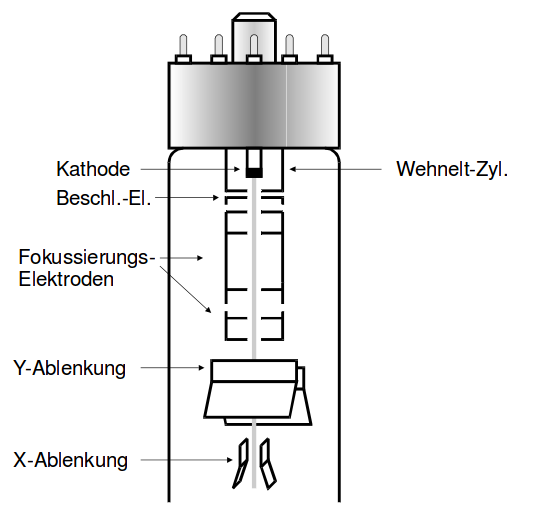
\includegraphics[height=6cm]{ressources/aufbau01.png}
  \caption{Grundlegender Aufbau einer Kathodenstrahlröhre. \cite{skript1}}
  \label{fig:aufbau1}
\end{figure}
Das Ziel des Gerätes ist es, freie Elektronen möglichst fokussiert zu beschleunigen.
Dazu werden zunächst Elektronen in einer Glühkathode freigesetzt.
Dies geschieht, indem ein Draht die Kathode indirekt heizt, so dass sich von dessen Oberfläche Elektronen herauslösen.
Damit dies auch bei niedrigen Temperaturen funktioniert, ist die Austrittsarbeit des Kathodenmaterials möglichst gering.
Durch eine Beschleunigungselektrode, an welcher durch die Beschleunigungsspannung $U_\text{b}$ ein positives Potential anliegt, werden die Elektronen beschleunigt.
Damit der Beschleunigungsvorgang ohne Kollisionen abläuft, muss sich die gesamte Kathodenstrahlröhre in einem Vakuum befinden.\\
Um den Beschleunigungsvorgang zu vereinfachen wird ein sogenannter Wehnelt-Zylinder verwendet.
An diesem liegt ein negatives Potential an, welches die Elektronen abstößt.
Dies führt einerseits zu einer Fokussierung des Strahls, da die Elektronen vom Kathodenrand abgestoßen werden, andererseits zu der Möglichkeit der Intensitätssteuerung des Elektronenstrahls.
Durch ein kleines Loch im Wehlent-Zylinder können die Elektronen die Glühkathode verlassen.
Mithilfe von Fokussierungselektroden, welche mit inhomogenen elektrischen Feldern arbeiten, wird der Strahl fokussiert.
Dies funktoniert ähnlich zur Optik, die Brechkraft der Fokussierung wird durch eine Spannung $U_\text{c}$ geregelt.\\
Nach der Fokussierung kann der Strahl durch zwei Kondensatorplatten, welche orthogonal zueinander in X-Richtung und Y-Richtung angeordnet sind, abgelenkt werden.
Dazu wird eine variable positive oder negative Ablenkspannung angelegt - Je nachdem, in welche Richtung der Elektronenstrahl wie stark abgelenkt werden soll.
Zum Schluss kann der Elektronenstrahl auf einem Leuchtschirm sichtbar gemacht werden.
Auf diesem treffen die Elektronen auf, so dass der Leuchtschirm zur Lichtemission angeregt wird.
Zudem ist ein Koordinatensystem mit 9 äquidistanten Linien im Viertelzollabstand eingezeichnet.

\subsection{Ablenkung des Elektronensrahls mit einem B-Feld}
Zur Untersuchung des Verhaltens des Elektronenstrahls unter Einfluss eines Magnetfeldes wird eine Helmholtz-Spule verwendet.
Diese bestehe aus zwei Kreisförmigen Spulen, die parallel angeordnet sind.
Genau in der Mitte beider Spulen entsteht somit ein nahezu homogenes Magnetfeld.
